% Graphical abstract (teaser) for manuscript.tex.
% Build: tectonic teaser.tex  -> figures/teaser.pdf (move or -o)
\documentclass[border=4pt]{standalone}
\usepackage{tikz}
\usetikzlibrary{arrows.meta,positioning,fit,calc}
\begin{document}
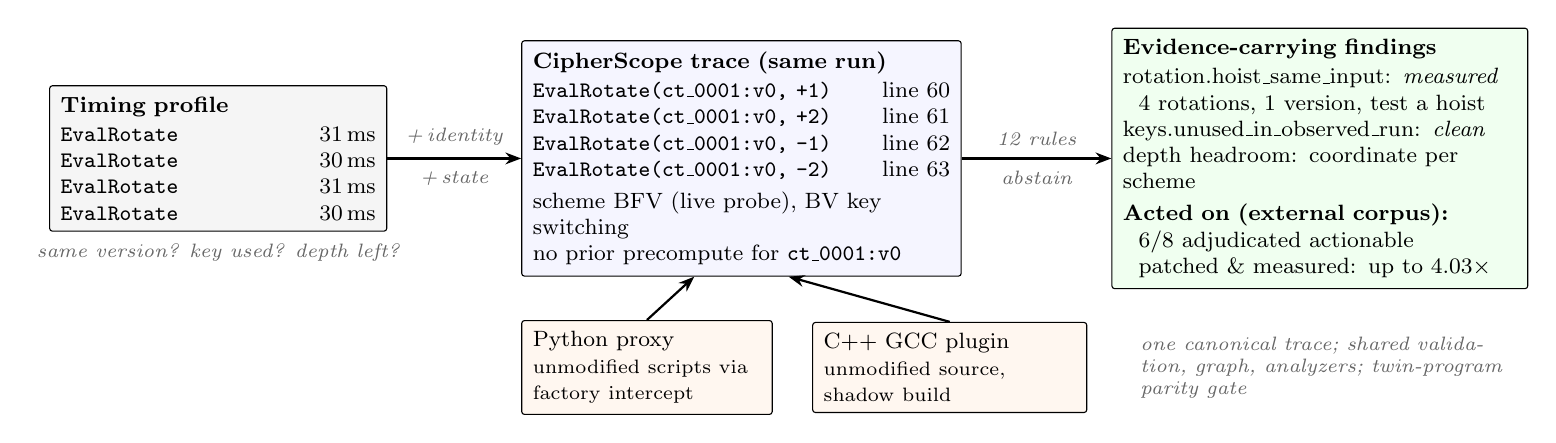
\begin{tikzpicture}[
      font=\footnotesize,
      box/.style={draw, rounded corners=1pt, align=left, inner sep=4pt, fill=blue!4},
      dim/.style={draw, rounded corners=1pt, align=left, inner sep=4pt, fill=black!4},
      finding/.style={draw, rounded corners=1pt, align=left, inner sep=4pt, fill=green!6},
      flow/.style={-{Stealth[length=2mm]}, thick},
      lbl/.style={font=\scriptsize\itshape, text=black!60}
    ]
    % Left panel: what a timing profile keeps
    \node[dim, text width=4.0cm] (prof) {
      \textbf{Timing profile}\\[1pt]
      \texttt{EvalRotate}\hfill 31\,ms\\
      \texttt{EvalRotate}\hfill 30\,ms\\
      \texttt{EvalRotate}\hfill 31\,ms\\
      \texttt{EvalRotate}\hfill 30\,ms
    };
    \node[lbl, below=1pt of prof] {same version? key used? depth left?};
%
    % Middle: CipherScope trace of the same run
    \node[box, right=1.7cm of prof, text width=5.3cm] (trace) {
      \textbf{CipherScope trace (same run)}\\[1pt]
      \texttt{EvalRotate(ct\_0001:v0, +1)}\hfill line 60\\
      \texttt{EvalRotate(ct\_0001:v0, +2)}\hfill line 61\\
      \texttt{EvalRotate(ct\_0001:v0, -1)}\hfill line 62\\
      \texttt{EvalRotate(ct\_0001:v0, -2)}\hfill line 63\\[2pt]
      scheme BFV (live probe), BV key switching\\
      no prior precompute for \texttt{ct\_0001:v0}
    };
%
    % Right: findings and measured outcome
    \node[finding, right=1.9cm of trace, text width=5.0cm] (find) {
      \textbf{Evidence-carrying findings}\\[1pt]
      rotation.hoist\_same\_input: \emph{measured}\\
      \ \ 4 rotations, 1 version, test a hoist\\
      keys.unused\_in\_observed\_run: \emph{clean}\\
      depth headroom: coordinate per scheme\\[2pt]
      \textbf{Acted on (external corpus):}\\
      \ \ 6/8 adjudicated actionable\\
      \ \ patched \& measured: up to 4.03$\times$
    };
%
    \draw[flow] (prof) -- node[above=1pt, lbl]{+\,identity} node[below=1pt, lbl]{+\,state} (trace);
    \draw[flow] (trace) -- node[above=1pt, lbl]{12 rules} node[below=1pt, lbl]{abstain} (find);
%
    % Frontends underneath
    \node[box, below=0.55cm of trace.south west, anchor=north west, text width=2.9cm, fill=orange!6] (py)
      {Python proxy\\ \scriptsize unmodified scripts via factory intercept};
    \node[box, right=0.5cm of py, text width=3.2cm, fill=orange!6] (cpp)
      {C++ GCC plugin\\ \scriptsize unmodified source, shadow build};
    \node[lbl, right=0.55cm of cpp, text width=4.6cm, align=left]
      {one canonical trace; shared validation, graph, analyzers; twin-program parity gate};
    \draw[flow] (py.north) -- ($(trace.south)+(-0.6,0)$);
    \draw[flow] (cpp.north) -- ($(trace.south)+(0.6,0)$);
  \end{tikzpicture}
\end{document}
